% Draft for review. Layout approximates the ACL two-column format with packages available
% locally; before submission, move the body into the official ACL template (acl.sty) and
% re-check the page count. Anonymous for review.
\documentclass[10pt,twocolumn]{article}
\usepackage[letterpaper,margin=2.5cm,top=2.5cm,columnsep=0.6cm]{geometry}
\usepackage{times}
\renewcommand{\ttdefault}{cmtt}   % Courier is not installed locally
\usepackage{microtype}
\usepackage{amsmath}
\usepackage{booktabs}
\usepackage{graphicx}
\usepackage[small,labelfont=bf]{caption}
\usepackage{xcolor}
\usepackage{url}
\usepackage[round]{natbib}
\usepackage[hidelinks]{hyperref}
\newcommand{\pending}[1]{\textcolor{red}{[#1]}}
\setlength{\parskip}{0pt}
\renewcommand{\arraystretch}{1.05}

\title{\Large Do Data Checks Tell You When to Trust a Text-to-SQL Answer?\\
A Pre-registered Study on Corrected BIRD Labels}
\author{Anonymous submission}
\date{}

\begin{document}
\maketitle

\begin{abstract}
A text-to-SQL system that answers wrongly should say so. Beyond model-based signals, a deployed
system can check an answer against the data with no model call: joins that count rows twice, results
cut off at a row limit, all-NULL aggregates, figures absent from the result. In a pre-registered study
on 393 held-out BIRD Mini-Dev questions, scored against corrected gold annotations, we ask how often
such checks apply and whether they warn as well as an LLM judge at the same flag rate. They apply to
only 4\% of answers, and there they catch no more errors than the judge with as many warnings (9 vs.\
10.8; 95\% CI of the difference $-6.3$ to $2.2$); they improve neither the judge's risk--coverage
curve nor a combined model. An agent retry is the most useful cheap warning (79\% precision).
Self-consistency and the judge rank answers about equally (AUROC 0.74 vs.\ 0.70, not significant). A
blind annotation of every error explains why checks rarely help: most errors are semantic.
With a second SQL model (exploratory) the checks again catch no more errors than the judge.
\end{abstract}

\section{Introduction}

Natural-language interfaces to databases are now good enough to deploy and still wrong often enough
to mislead. A business user who asks how many patients had an abnormal test and receives a confident
number cannot tell whether the query counted patients or lab tests. An honest ``this might be wrong''
attached to such answers is worth more than a slightly higher accuracy.

Two families of signals can provide it. \emph{Model-based} signals ask a model again: resample the
query and measure agreement (self-consistency), or ask a separate LLM to judge the answer; recent work
places black-box signals around 0.61--0.68 AUROC and LLM judges at 0.72--0.78
\citep{richardson2026predicts}. \emph{Data checks} inspect the answer against the database with no
model call. They are free, instant and explainable (``this join repeats each patient 46 times''),
which makes them attractive in a product.

We built such checks into a self-hosted text-to-SQL system and asked, in a pre-registered study,
whether they earn their place. Our contributions:
\begin{enumerate}\setlength{\itemsep}{0pt}
\item A pre-registered comparison of data checks, process signals, LLM judges and self-consistency as
correctness warnings on 393 held-out BIRD Mini-Dev questions \citep{li2023bird} scored against
corrected annotations \citep{jin2026annotation}, with a matched-flag-rate primary measure that is fair
to rarely-firing yes/no checks.
\item A blind error-type annotation of every wrong answer (two annotators, $\kappa=0.74$) with a catch
matrix of which signal sees which error.
\item A negative result with its reason: data checks rarely apply and do not beat a judge or
self-consistency, because most errors are semantic; structural double-counting checks miss double
counting that happens through legitimate joins.
\item A frozen fan-out question set (60 risky, 33 control) on which current models rarely double count
(0 and 5 of 60), and a second-model replication of the main results.
\end{enumerate}

\section{Related work}

\textbf{Correctness prediction.} \citet{richardson2026predicts} compares black-box, white-box and
verification signals on BIRD and Spider; \citet{somov2025confidence} study entropy-based selective
classifiers; \citet{chen2025abstention} add abstention via conformal prediction on hidden states. All
of these signals come from a model. \textbf{Database feedback.} SQLens \citep{gong2025sqlens} is the
closest work: it combines database signals (abnormal results, empty predicates, join-tree issues) with
LLM signals in a learned classifier. We instead evaluate data checks as warnings in their own right,
at a matched flag rate, on corrected labels, with pre-registered hypotheses and an error annotation
that explains what the checks can and cannot see. \textbf{Benchmark quality.}
\citet{wretblad2024noise} document noise in BIRD; \citet{jin2026annotation} report annotation errors
in 52.8\% of Mini-Dev and release corrections, which we score against. Execution match has false
negatives \citep{pourreza2023evaluating,kim2025flex}; we quantify them after correction.
\textbf{Self-consistency} \citep{wang2023selfconsistency} is applied here as agreement between the
execution results of resampled queries.

\section{System and signals}

The system routes each question; for database questions an LLM writes SQL, a read-only gate validates
it, and it runs with a row cap. The model retries with a classified error message when a query fails
or returns nothing; a second call writes the answer from the first rows of the result. SQL and answers
are written by GPT-5 mini at its provider's default sampling (it accepts no temperature), reached
through the Zed editor's hosted-model service via a local OpenAI-compatible proxy; Qwen3.8-27B (Groq,
temperature 0) normalises the question. The served model is recorded on every call.

\textbf{Data checks} (no model call): a \emph{fan-out probe} compares \texttt{COUNT(key)} with
\texttt{COUNT(DISTINCT key)} per joined table for aggregates over joins; \emph{truncation} (the result
hit the row cap); \emph{NULL-heavy} (an all-NULL aggregate); \emph{figure grounding} (every number in
the answer must trace to a result cell, a column aggregate, the question, or the number of rows shown
to the answer writer); and \emph{any data check}, their union. \textbf{Process baselines}: the query
failed, the result was empty, the agent needed a retry, the answer refuses. \textbf{Model baselines}:
an LLM judge (Gemini 3.8 Flash via the same service, primary; gpt-oss-120b, secondary; their mean as
an ensemble), each
from a different family than the SQL model and shown the question, schema, SQL, first rows and answer;
and self-consistency (five resamples of the SQL call, each executed; risk is the share whose result
differs from the answer's).

\section{Study design}

\textbf{Pre-registration.} The protocol was written before measuring. A 100-question pilot exposed
harness faults (a prompt rule that turned \texttt{LIMIT 1} into \texttt{LIMIT 1000}; grounding false
alarms from the pipeline's own wording; noisy original labels), and the protocol was revised before
any held-out question was asked. Pilot questions are development data, excluded from all results;
every amendment is logged with whether the pilot informed it.

\textbf{Data.} Mini-Dev has 498 unique questions; the 398 outside the pilot, minus 5 whose SQLite and
PostgreSQL copies disagree on the original gold, form the held-out set of 393. Labels are the
corrected annotations \citep{jin2026annotation}, written for SQLite: gold runs on BIRD's SQLite
databases, predictions on the PostgreSQL copy, compared to five significant digits (validated on the
original golds of both copies: 491 of 498 agree). The \textbf{fan-out set} has 60 risky questions,
whose natural SQL aggregates a parent-level quantity across a one-to-many join, and 33 controls on the
same tables; each has a gold query, an independently written check query that must agree with it, and
the naive join, which must differ from gold (risky) or equal it (control). It was drafted with an AI
assistant from rules fixed in advance and frozen after the author reviewed a random 20\%.

\textbf{Measures.} The SQL label is execution match (relaxed: column order and extra columns ignored;
BIRD's strict rule also reported). The \emph{primary measure} is wrong answers caught at a matched
flag rate: when a signal flags $k$ answers, we compare its wrong answers with the expected number among
the judge's $k$ most suspect (ties broken at random, computed exactly). We also report precision,
recall, AUROC and the area under the risk--coverage curve (AURC). Statistics use a paired bootstrap
stratified by database (2,000 resamples) and Holm correction over four confirmatory tests: \textbf{H1}
the fan-out check beats the judge at its flag rate on the fan-out set; \textbf{H2} ordering by any
data check, then judge risk, lowers the judge's AURC; \textbf{H3} grounding flags fewer than 5\% of
correct answers; \textbf{H4} one evidence-guided repair fixes more than it breaks and adds 2 points.
H1 and H4 require at least 10 double-counting errors or repairs, else they are untestable; if the main
model fails H1's precondition, the set is rerun with a second model (gpt-oss-120b). Every wrong answer
was annotated blind to the signals into ten types; a second annotator (another model, on a reshuffled
blank copy) labelled all 90 ($\kappa=0.74$; 0.87 for system error vs.\ benchmark artefact).

\section{Results}

\textbf{Accuracy.} 77.1\% under the relaxed rule (95\% CI 72.5--81.2; strict 70.2\%); against the
original gold, 66.4\%. Counting the 20 errors whose only fault is output format as correct gives
82.2\% (exploratory).

\begin{table}[t]
\centering\small
\setlength{\tabcolsep}{3.5pt}
\begin{tabular}{lrrrr}
\toprule
signal & $k$ & prec. & rec. & vs.\ judge at $k$ (95\% CI) \\
\midrule
any data check & 17 & .53 & .10 & $-1.8$ ($-6.3$, $2.2$) \\
\quad fan-out & 1 & 1.00 & .01 & $+0.4$ \\
\quad truncation & 9 & .22 & .02 & $-3.7$ ($-7.4$, $-0.7$) \\
\quad NULL-heavy & 2 & 1.00 & .02 & $+0.7$ \\
\quad grounding & 5 & .80 & .04 & $+0.8$ ($-1.2$, $2.8$) \\
query failed & 4 & 1.00 & .04 & $+1.5$ ($0.4$, $2.9$) \\
empty result & 6 & 1.00 & .07 & $+2.2$ ($0.7$, $4.1$) \\
needed a retry & 24 & .79 & .21 & $+3.7$ ($-1.7$, $8.6$) \\
refusal & 7 & .57 & .04 & $-0.5$ ($-2.7$, $1.7$) \\
\bottomrule
\end{tabular}
\caption{Warnings on the held-out set (90 of 393 wrong). Last column: wrong answers the signal catches
minus the judge's expected catch among its $k$ most suspect answers. Failed and empty queries are wrong
by construction here: no corrected gold result is empty.}
\label{tab:signals}
\end{table}

\begin{figure}[t]
\centering
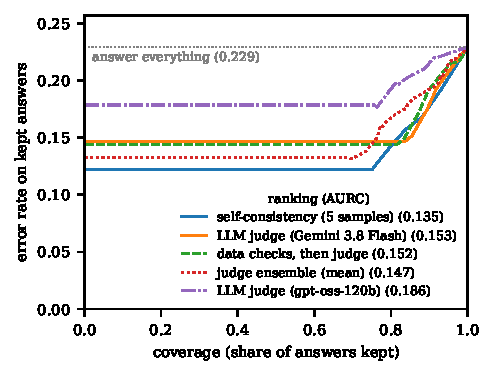
\includegraphics[width=\columnwidth]{../fig_risk_coverage.pdf}
\caption{Risk--coverage on the held-out set. Flat segments are large ties: most answers get the
lowest risk from every ranking.}
\label{fig:rc}
\end{figure}

\textbf{Warnings} (Table~\ref{tab:signals}). The data checks fire on 17 answers (4\%) and catch 10\%
of the errors, slightly fewer than the judge's 17 most suspect answers (9 vs.\ 10.8). An agent retry
is a stronger cheap warning: retried answers are wrong 79\% of the time, a fifth of all errors. Failed
and empty queries are always wrong here, but only by construction (no corrected gold result is empty;
in deployment an empty result can be right). Self-consistency (AUROC 0.739) and the Gemini judge
(0.697) rank answers about equally: the difference is not significant (95\% CI $-0.03$ to $0.11$) and
disappears when the 20 format-only errors count as correct (0.761 vs.\ 0.757), because resampled
queries vary in format and so flag answers the scorer wrongly marks wrong. The judge ensemble reaches
0.701 and the gpt-oss judge 0.606 (Figure~\ref{fig:rc}). The judge is tie-heavy ($p=1$ for 328 of 393
answers); ties are broken at random in expectation.

\textbf{Hypotheses.} \textbf{H2 is not supported}: AURC gain 0.001 (95\% CI $-0.005$ to $0.009$,
$p=0.42$). \textbf{H3 is supported} (2 of 242 correct answers flagged; upper bound 2.6\%,
$p=0.0004$), but grounding fired on only 5 answers, and 3 of its 4 hits are failed queries whose text
quotes an error code. \textbf{H4 is untestable}: 2 repairs were triggered. \textbf{H1}: see below.
After Holm correction over the testable hypotheses (H2, H3), only H3 is supported.

\begin{table}[t]
\centering\small
\setlength{\tabcolsep}{3pt}
\begin{tabular}{lrrrrr}
\toprule
error type & $n$ & checks & empty & retry & judge \\
\midrule
filter value & 22 & 3 & 3 & 5 & 6 \\
output format only & 20 & 1 & 0 & 3 & 1 \\
column meaning & 15 & 1 & 2 & 5 & 2 \\
aggregation & 8 & 1 & 0 & 1 & 0 \\
hint contradicts data & 8 & 0 & 0 & 0 & 0 \\
ordering / top-$k$ & 6 & 0 & 0 & 0 & 1 \\
other (4 failed SQL) & 6 & 3 & 1 & 5 & 1 \\
double counting & 4 & 0 & 0 & 0 & 1 \\
gold error & 1 & 0 & 0 & 0 & 0 \\
\bottomrule
\end{tabular}
\caption{The 90 wrong answers by type, and how many each signal flags (judge: its 17 most suspect,
the data checks' flag rate).}
\label{tab:errors}
\end{table}

\textbf{What the errors are} (Table~\ref{tab:errors}). Most errors are semantic: a wrong filter
value, a plausible but wrong column, an aggregate answering a neighbouring question. The fan-out probe
caught none of the four double-counting errors: three count the wrong entity through a join that is
itself legitimate (lab rows instead of patients, result rows instead of drivers, rulings across card
printings), and one repeats rows inside a subquery the probe does not parse. A fifth of the errors are
formatting differences (a fraction for a percentage, a timestamp for a date).

\textbf{Fan-out set.} GPT-5 mini answered 59 of 60 risky questions correctly and never double
counted: 39 of its queries use \texttt{COUNT(DISTINCT)} and 15 a semi-join; the one wrong answer is a
semi-join that failed on a malformed column name. H1's precondition fails for this model, so the set
was rerun with gpt-oss-120b (temperature 0): 54 of 60 risky questions correct and 5 double-counting errors, still
short of 10, so \textbf{H1 is untestable} for both models. Exploratory: the fan-out check fired on 4
answers, all wrong (4 of the 5 double counts, no false alarms); the judge's 4 most suspect answers
catch 3.2, but 6 answers came back from the host with empty text, and without them the judge ties the
check (4 vs.\ 4).

\textbf{Run-to-run variation.} Fifty random held-out questions asked a second time changed label on 5
(10\%; 95\% CI 3--22\%): four became correct, one became wrong; signals changed on at most 2. All five
flipped questions had first-run self-consistency risk of at least 0.4 (mean 0.76, vs.\ 0.09 for the
45 stable ones; exploratory). This is close to expected by construction: a second run is one more
sample from the same distribution, so answers flip where samples disagree.

\textbf{Exploratory: combining signals.} Decided after the confirmatory results and labelled as such.
A logistic regression over all signals, scored out-of-fold, reaches AUROC 0.785 (AURC 0.122); without
the data checks it reaches 0.801 (0.103), so the checks add nothing jointly either. Judge plus
self-consistency alone gives 0.790, and the free signals alone 0.578. Acting on warnings (re-running or
replacing a doubtful answer) is studied separately.

\textbf{Exploratory: a second SQL model.} Decided after the confirmatory results. We repeated the
held-out run with gpt-oss-120b at its provider's default sampling, as for GPT-5 mini (a first run sent
temperature 0, which made its self-consistency samples near-copies; it is superseded). Accuracy is
75.8\%. The data checks flag 22 answers (6\%) and catch 9 errors, against 12.3 for the judge at the same
flag rate (difference $-3.3$, 95\% CI $-9.0$ to $1.7$). Ordering by the checks first does not improve
the judge's curve (AURC gain 0.002, CI $-0.007$ to $0.014$), and the combined model is better without
them (AUROC 0.792 vs.\ 0.774). The agent retry again leads the cheap signals (26 flags, 69\% precision;
$+3.4$ over the judge, CI $-1.5$ to $8.3$). Self-consistency and the judge again rank about equally
(AUROC 0.715 vs.\ 0.683; difference $+0.03$, CI $-0.05$ to $0.11$); 38 of the 95 wrong answers had five
agreeing samples (40\%, as for GPT-5 mini). The host returned an empty answer text on 39 answers (35
with correct SQL), which the judge, shown the text, rated lower; without them its AUROC is 0.713 and
self-consistency's 0.725. Figure grounding raised 3 false alarms on 207 correct texts; 7 repairs
triggered, so H4 stays untestable.

\section{Discussion}

\textbf{Why data checks rarely help.} The checks see the query and its own result, while most errors
are about meaning. A result can be internally consistent and still answer the wrong question. Even
double counting mostly happens through joins that are correct for some reading of the question:
``count lab rows'' and ``count patients'' share a join, and only the question says which was meant. Current
models also rarely fall into the textbook fan-out trap the probe was built for (0 and 5 of 60 risky
questions), and when one does, a strong judge notices too.

\textbf{What works cheaply.} An agent retry costs nothing and catches a fifth of the errors at 79\%
precision. Self-consistency and an LLM judge rank answers similarly; self-consistency costs five extra
calls (two thirds of our generation cost) and partly flags scorer false negatives. A second SQL model
gives the same ordering. In a product we would show the retry signal and a judge, and keep data checks as explanations
attached to a flagged answer rather than as detectors.

\textbf{What the benchmark measures.} Scoring against the corrected gold moves accuracy by 10.7
points (part of this comes from the 81 questions the correction file rewords); even after
correction a fifth of the remaining errors are formatting, and 8 involve a hint that contradicts the
data or the gold. Running a SQLite benchmark on its PostgreSQL copy adds artefacts (7 of 498 golds
disagree; PostgreSQL sorts NULLs first in descending order, which turned 2 answers wrong), and the
released correction file rewords 81 questions and 68 hints. Studies of warning signals on BIRD should
use corrected labels and, ideally, an answer-level label.

\section*{Limitations}

One SQL model in the confirmatory study (GPT-5 mini, provider default sampling), with a second model
(gpt-oss-120b) only as an exploratory replication; both may have seen BIRD in training. GPT-5 mini and
the Gemini judge were reached through an editor's hosted-model service rather than the providers' own
APIs, so provider-side settings could not be inspected. The checks' coverage, not only their accuracy,
limits what our tests could show: they fired on 17 answers. Both error annotators are models, blind to the signals; the author reviewed the labels of 18 sampled
answers (not blind) and agreed with them, but no independent human annotation was made. The fan-out set follows a textbook pattern and was drafted with an AI assistant; its null result
says nothing about subtler double counting. Free-tier limits forced a change of host for the
gpt-oss-120b runs to a reseller that does not disclose its upstream; we checked the served model on
every call and that the reasoning-effort setting was honoured, and the secondary judge's verdicts
agree with the original host's on 93\% of 260 shared answers (AUROC 0.62 vs.\ 0.63). Its normaliser made the same language decisions as Groq's on 17 of 17 dev questions but passed two
fewer name hints. The same host returned an empty answer text on 6 of the 93 robustness answers and 39 of the 393 replication answers; their SQL labels are unaffected, and
we report the judge comparison with and without them. English questions, one benchmark, the SQL path
only.

\section*{Ethics and disclosure}

BIRD Mini-Dev and the corrected annotations are CC BY-SA 4.0. The protocol, frozen samples (with
hashes), run records (served model per call), scorer and analysis will be released. An AI assistant
helped write code, annotate errors blind to the signals, and draft this text; the authors reviewed
all outputs and take responsibility for them.

\bibliographystyle{plainnat}
\bibliography{refs}

\end{document}
